% DEFINED:   sec:bengio-alice, fig:ch04-lm-loss
% RESOLVED:  (none new)
% FORWARD:   sec:window-limits (Task 6)

\section{The experiment: char-level Alice}\label{sec:bengio-alice}

The corpus is the first $30{,}000$ characters of \emph{Alice's Adventures
in Wonderland}, a $75$-character vocabulary at the character level. The
same corpus and vocabulary feed the next chapter's recurrent network, so
the two models are compared on identical data. The configuration is small
on purpose:
\begin{itemize}
\item context $N = 8$ characters (each example is eight ids in, one id out),
\item embedding dimension $d = 16$,
\item hidden layer $h = 64$ units,
\item SGD at learning rate $0.02$, batch size $1$,
\item $4$ epochs over the corpus.
\end{itemize}
Sliding the window over the corpus gives $29{,}992$ training examples. The
parameter count is
\[
  75 \cdot 16 + 8 \cdot 16 \cdot 64 + 64 + 64 \cdot 75 + 75
  \;=\; 14{,}331,
\]
the embedding table, the first \texttt{Linear} and its bias, and the
second \texttt{Linear} and its bias.

A model that predicts the next character uniformly at random scores
$\log 75 \approx 4.32$ nats per character, the entropy of the uniform
distribution over the vocabulary. That is the baseline to beat. Over the
four epochs the mean per-character loss falls
\[
  4.32 \;\to\; 2.57 \;\to\; 2.22 \;\to\; 2.11 \;\to\; 2.04
\]
nats per character, ending at $2.04$ (perplexity $e^{2.04} \approx 7.67$).
\Cref{fig:ch04-lm-loss} plots the trajectory. Most of the gain arrives in
the first epoch, where the model learns character frequencies and the
commonest short patterns; the later epochs sharpen word boundaries and
local agreement.

\begin{figure}[ht]
  \centering
  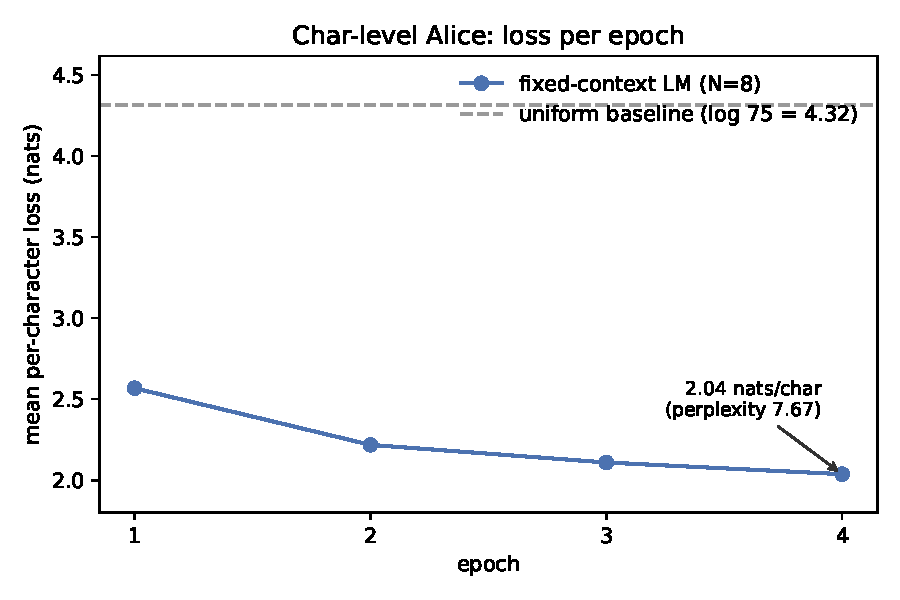
\includegraphics[width=0.7\linewidth]{figures/ch04-lm-loss.pdf}
  \caption{Char-level Alice: mean per-character loss per epoch for the
    fixed-context language model ($N = 8$, $d = 16$, $h = 64$). The dashed
    line is the uniform-random baseline, $\log 75 \approx 4.32$ nats per
    character. In four epochs over $29{,}992$ eight-character windows the
    loss falls to $2.04$ nats per character (perplexity $7.67$), which is
    $2.94$ bits per character. The steep first epoch is the model learning
    character frequencies and the commonest short patterns; the flatter
    tail is local agreement being sharpened.}
  \label{fig:ch04-lm-loss}
\end{figure}

\textbf{What the samples look like.} Sampling from the model at each epoch,
seeded with \texttt{"alice was "} and drawn at temperature $0.8$, shows the
trajectory directly (the paired notebook stores the full samples). After
one epoch the output is the right letters in the wrong order, with a few
real words surfacing: spacing and common short tokens like \texttt{the} and
\texttt{to} appear, but most of the stream is plausible-looking nonsense.
By the fourth epoch the fragments are English-shaped, with recognizable
words (\texttt{the}, \texttt{was}, \texttt{and}, \texttt{her}, \texttt{of})
and occasional plausible phrases, though punctuation and quotation balance
stay hopeless and there is no coherence beyond a few characters. Character
names other than \texttt{Alice} do not reliably appear, which is exactly
what an eight-character window predicts: a name introduced hundreds of
characters earlier is long gone from the model's input.

\textbf{The compression reading.} The per-character cross-entropy in nats
converts directly to bits per character, $2.04 / \ln 2 \approx 2.94$ bits
per character. That number is the model's compression rate on this corpus,
and the identity is not an analogy. Cross-entropy in bits per character
\emph{is} the expected code length per character under a Shannon-optimal
code built from the model's predictive distribution $p_\theta$. A model
that predicts better assigns higher probability to what actually comes
next, which is the same thing as encoding it in fewer bits. This is the
chapter's north star, the thread that runs from prediction to compression
and back: learning a good language model and finding a good code for the
data are one problem viewed from two sides, and the bibliographic notes
trace the lineage from Shannon's entropy of English to the
minimum-description-length and Solomonoff view of induction. The
Transformer chapter returns to this same bits-per-character measure when it
asks what a better architecture buys.
